\documentclass[tikz]{standalone}
\begin{document}
    \usetikzlibrary{shapes,arrows,positioning,automata}
    \usetikzlibrary{matrix,arrows,decorations.pathmorphing}
    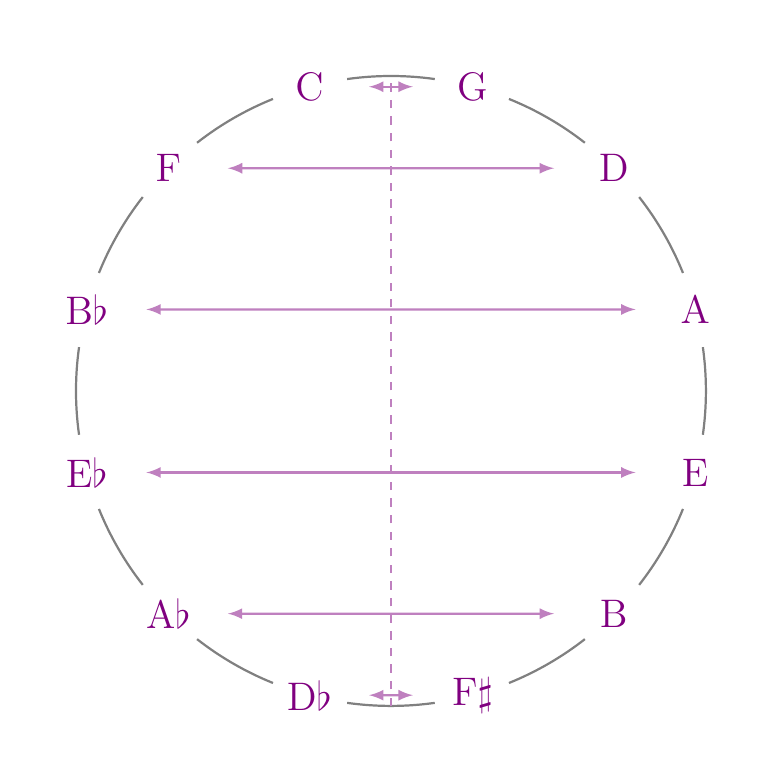
\begin{tikzpicture}[auto,node distance=2.5cm, block/.style={color=black, align=center, minimum height=1cm, minimum width=1.5cm}, vec/.style={thick,color=black!50}]

        \def \n {12}
        \def \radius {4 cm}
        \def \margin {7}

        \def \notes {-5/D$\flat$, -4/A$\flat$, -3/E$\flat$, -2/B$\flat$, -1/F, 0/C, 1/G, 2/D, 3/A, 4/E, 5/B, 6/F$\sharp$}

        \foreach \s/\key in \notes {
          \def \start {360 * \s / \n + 15}
          \def \end {360 * (\s - 1) / \n + 15}

          \node[block, circle, color=violet] at ({90-\start}:\radius) (a\s) {\Large\key};
          \draw[vec] ({\end+\margin}:\radius) arc ({\end+\margin}:{\start-\margin}:\radius);
        }

        \draw [thick,dashed,color=violet!50] (0, -\radius) -- (0, \radius);

        \draw[latex-latex,color=violet!50,thick] (a0) to (a1);
        \draw[latex-latex,color=violet!50,thick] (a2) to (a-1);
        \draw[latex-latex,color=violet!50,thick] (a3) to (a-2);
        \draw[latex-latex,color=violet!50,thick] (a4) to (a-3);
        \draw[latex-latex,color=violet!50,thick] (a5) to (a-4);
        \draw[latex-latex,color=violet!50,thick] (a6) to (a-5);

    \end{tikzpicture}
\end{document} 
